\section{Simulation of the Scheme}
In order to do a preliminary evaluation of the effectiveness of the scheme presented in section \ref{sec:DPLC}, a simulation of the behavior in a BSC with a bit error probability of $0.01$ is performed. This is the same channel model as in section \ref{sec:pacSizeInf}, where the theoretical best packet length was found to be 39 bytes, i.e. 28 bytes of payload and 11 bytes of header. 
The simulation allows payloads of length $l_i \in \{10, 20, ... , 100\}$, $\forall i$. Initially, $l_0 = 10$, $l_1 = 20$ and $\mathcal{E}_0 = 0$. For each time step, transmission of $N_{\text{packets}}$ are simulated. If one or more bit errors occur in a packet, it is considered dropped. The PRR are then calculated as the ratio of non-dropped packets against the number of sent packets. The current transmission efficiency is found according to equation (\ref{E}). From this, the value of $d$ is calculated according to equation (\ref{eq:d}), and finally the new packet length is chosen based on the intervals defined in figure \ref{fig:d}, where $D=0.1$, i.e. a $1 \%$ increase or decrease in efficiency is required for the payload length to be adjusted. If the change is less than this, the packet length remains the same, and the transmitter is considered in steady state for $3$ time steps, after which $10$ bytes is added to the payload length if the payload size is not already at maximum, $100$, where $10$ bytes will be subtracted.
\\[8pt]
\begin{figure}
\centering
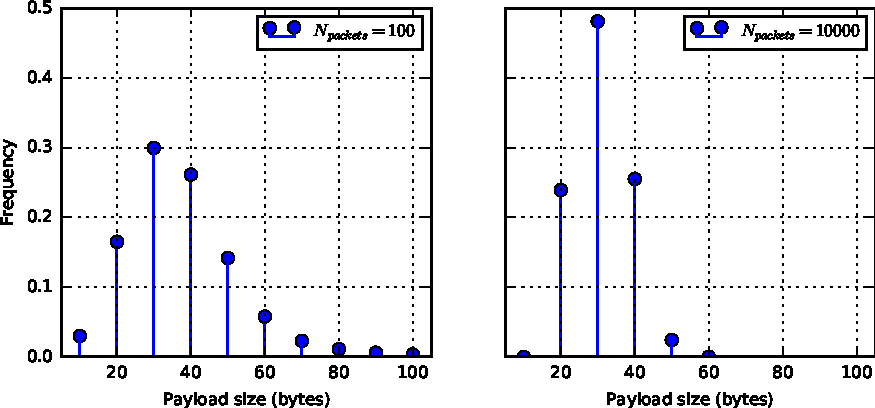
\includegraphics[scale=1]{figs/DPLCsim.pdf} 
\caption{\textit{Frequency of payload lengths chosen in simulation of dynamic scheme, with $N_{\text{packets}}$ used for estimating PRR each time slot.
Left: $N_{\text{packets}}=100$. Right: $N_{\text{packets}} = 10000$}\label{fig:DPLCsim}}
\end{figure}
The results of performing this simulation can be seen on figure \ref{fig:DPLCsim}. Here, two different scenarios are illustrated by histograms with the frequency that each packet length is chosen. The left figure shows the result for $100$ packets used to estimate the PRR in each time step. It is seen that the most used payload sizes are $20-50$ bytes, with $30$ and $40$ most frequent. By inspection of figure \ref{fig:BSC}, this is reasonable: There is some difference in the theoretical efficiency within this interval, but it is not very large. However, it is seen that larger payload lengths are also chosen occasionally. The reason for this can be explained by the stochastic behavior in the channel. Even though the theoretical efficiency is know and the channel is not time-varying, the estimates at given time steps could be wrong, causing the scheme to choose these payload lengths. In contrary, the right figure shows the result of using $10000$ packets to estimate the PRR at each time step. Here, the result is clearer: Payloads of $20-40$ bytes are chosen $97.5\%$ of the time and a payload length of $30$ is chosen $48\%$ of the time. This is a nice result when the theoretical best payload is $28$ bytes, but may not be very useful in practice, since real channels are time-varying, and using so many packets to estimate the PRR may not be feasible, since the channel could change in this time.

